\documentclass[dvipdfmx, openany,10pt]{jsarticle}
\usepackage{graphicx}    % 画像挿入用
\usepackage{amsmath}     % 数式
\usepackage{amssymb}     % 数式記号
\usepackage{bm}          % 太字ベクトル
\usepackage{cite}        % 文献参照の整形
\usepackage{hyperref}    % 目次やリンク
\usepackage[version=3]{mhchem}

\begin{document}
\title{生体医工学Ⅰ 課題レポート}
\author{}
\date{2025年7月9日}
\maketitle
{\small\section{医薬品の探索について熱力学的解析・速度論的解析が重要な指標になる理由}}
医薬品の探索において標的となる分子について物理化学的なアプローチを用いることによって,標的分子とリガンドの間での結合における固有な特徴を解析することができ,その結果として医薬品の有効な設計につながると考えられる。
ITC(等温滴定型カロリメトリー)は、タンパク質とリガンドとの間に生じる結合反応に伴う熱変化を直接測定する手法である。薬剤探索や分子間相互作用の研究において極めて重要な技術である。\\
この測定により得られる代表的なパラメータには、まず解離定数を示す$k_{\text{d}}$がある。これはリガンドが標的タンパク質とどれほど強く結合するかを示していて、値が小さいほど結合親和性が高いことを意味する。
次にエンタルピー変化である$\Delta H$は、結合に伴う発熱あるいは吸熱を表し、水素結合、疎水性相互作用、イオン相互作用などの物理的要因が明らかとなる。
エントロピー変化を示す$\Delta S$は、結合によって分子の秩序や自由度がどう変化したかを示し、疎水効果性相互作用を反映する。\cite{長門石曉2020医薬品}
これらから算出されるギブス自由エネルギー変化である$\Delta G$は、結合の自発性や安定性を定量的に評価する指標である。ここで$\Delta G$は,
\[ \Delta G = \Delta H - T\Delta S \]
と表される。例えば$\Delta H$と$\Delta S$が$\Delta G$に与える影響の大きさを考えることによって,標的分子とリガンドの間の結合様式の特徴を捉えることができると考えられる。さらに,タンパク質1分子に対して何分子のリガンドが結合しているかが分かる。
創薬において、これらの情報は不可欠である。リガンドが標的タンパク質に結合しているかどうかを直接的かつ定量的に確認できるほか、結合の強さや結合様式の違いを比較検討するために用いられる。
ITCは実験操作が比較的単純でありながら、結合の親和性、熱力学的性といった複数の重要なパラメータを同時に得ることができる。
これにより、構造最適化、薬剤の選択性評価、結合メカニズムの解明、血中タンパク質との非特異的結合の評価などが可能となる。\\
\indent 一方で速度論的解釈によって,標的分子とリガンドの間のresidence timeを測定することが可能となり,その結果として薬効の持続性を調べることができる。滞在時間は薬が標的にどれだけ長く結合しているかを示しており,体内から薬が排出された後でも薬の効果が継続する現象の説明などとなる。
従来医薬品の薬効を図る指標として結合次数というものが存在していた。標的分子とリガンドの間での平衡反応を以下のように仮定したときの結合次数はさらに以下のようになる。\\
\[ \ce{R + L <=>C[k_{\text{on}}][k_{\text{off}}] RL} \]
\[ k_d = \frac{k_{\text{off}}}{k_{\text{on}}} = \frac{[R][L]}{[RL]} \]
実験的にこの$k_d$は$k_{\text{off}}$の影響を受けやすいとわかっている。\cite{copeland2016drug}また,上記のような平衡が成立していると考えると,持続時間は以下のようにわかる。
まず,この解離反応は一次反応とみなされ、そのresidence time(滞在時間)は指数分布に従う。時刻 $t$ にもまだ解離していない確率は次の通り:

\[
P(t) = e^{-k_{\text{off}} t}
\]

このとき、平均滞在時間(residence time)$\tau$ は期待値として以下のように定義される:

\[
\tau = \mathbb{E}[t] = \int_0^\infty t \cdot k_{\text{off}} e^{-k_{\text{off}} t} \, dt
\]
したがって、
\[
\tau = \frac{1}{k_{\text{off}}}
\]
\indent 以上を踏まえると$k_d$は$k_{\text{off}}$に比例し,$k_{\text{off}}$は$\tau$を導くので,$k_d$のみを調べればいいと考えてしまうが,上記の平衡反応が多段階で起きている場合等は$k_d$から滞在時間までを直接推測することは困難である。\\
そこでSPR測定等の技術を用いて$\tau$を直接測定することに意義があると考えられる。例えばFabl還元酵素阻害剤は$\tau$と薬効の間に強い相関があるとわかっている。\\
以上踏まえると,速度論的解析を通して$\tau$を直接計測することに意義があり,そのことによって,
\begin{itemize}
  \item 薬効の持続性を知る
  \item 少ない投与回数での薬の効果を発揮する
  \item off-targetを防ぎ,副作用を防ぐ
\end{itemize}
等といったことができると考えられるので,速度論的解析は重要な指標となる。
{\small\section{低分子医薬品・抗体医薬品について医薬品開発を目指す際のアドバンテージおよび懸念点}}
低分子医薬品の特徴は分子量が$500Da$以下で,化学合成によって作られる有機化合物であり,主に経口投与ができるという特徴があり,細胞内,細胞外両方の標的に到達可能である。
アドバンテージとしては細胞内の酵素や受容体に容易に到達できるので,標的分子に特異的に結合するように製造することが比較的容易であることや,化学合成で製造するため,比較的安価で大量に生成しやすいことが挙げられる。
一方で懸念点としては類似構造の他の分子に反応してしまって副作用を生じてしまうことや長期間の使用により標的分子に変異が生じて,医薬品が効かなくなることなどが挙げられる。\\
\indent 抗体医薬品は、体内の免疫が持つ抗体の仕組みを応用したタンパク質製剤である。これは、がんや自己免疫疾患など、特定の病気の原因に特異的に作用する。高い効果が期待でき、副作用が比較的少なく、作用時間が長いのが特徴である。
製造は、まず抗体の遺伝子であるDNAを設計するところから始まる。これを、主にCHO細胞といった哺乳類細胞に組み込む。遺伝子が組み込まれた細胞は、バイオリアクターという装置の中で大量に培養され、抗体を分泌する。
培養液から抗体を回収した後、クロマトグラフィーといった方法で精製し、最後に無菌状態で薬剤として形を整える。この薬剤はタンパク質であり,消化酵素によって分解されてしまうので,口から飲むことはできず、注射や点滴で投与される。\\
\indent 懸念点としては,高い特異性と治療効果が見込める一方で、製造には多額のコストがかかる。また、タンパク質からなるため,変性を防ぐための温度管理や無菌状態の維持などの管理が求められ、さらに、体に免疫反応が起こる、免疫原性のリスクもあるといった課題を抱えている。

{\small\section{タンパク質の図示}}
AlphaFold Serverを用いて調べた。
\begin{figure}[htbp]
 \begin{center}
  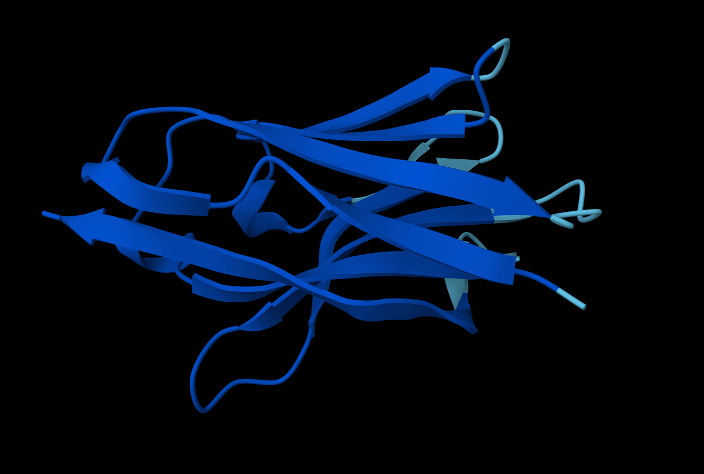
\includegraphics[width=100mm]{alphafold.png}
 \end{center}
 \caption{AlphaFoldを用いて得たタンパク質の構造}
 \label{fig:one}
\end{figure}

\bibliographystyle{jplain}
\bibliography{bio}

\end{document}
